As already mentioned, there have been 3 independent earthquakes, as could be 
seen in Figure~\ref{fig:eq_start_heat}: Apr 6th 2:00~PM, Apr 8th 7:00~AM and Apr 
9th 3:00~PM, approximately. Those two last earthquakes are emphasized in
Figure~\ref{fig:eq_2_3_heat}.

\begin{figure}[!h]
    \centering
    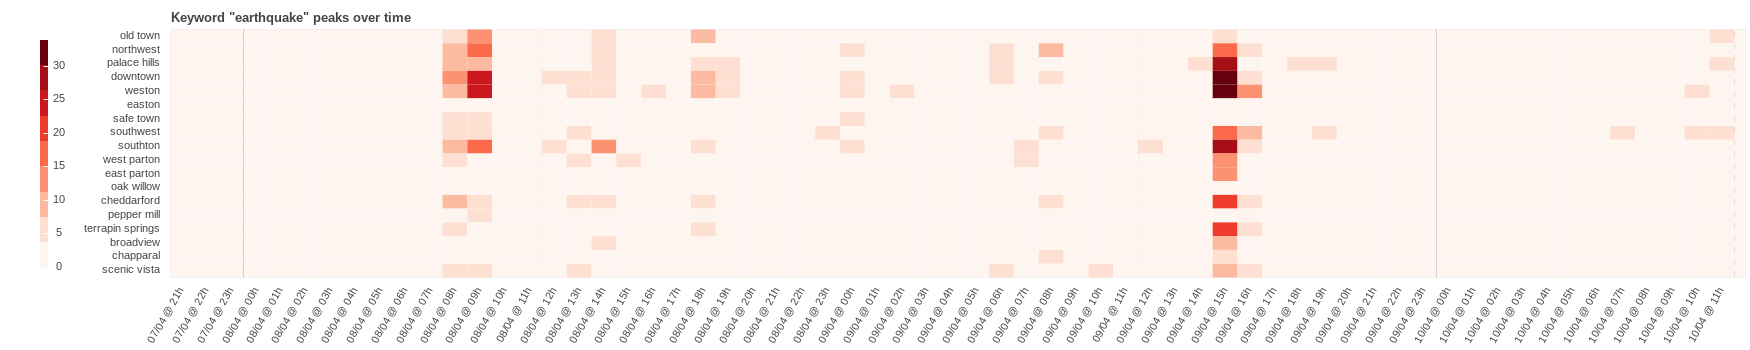
\includegraphics[width=1.00\textwidth]{figs/q2/eq_2_3_heat}
    \caption{Heatmap for the two last earquakes using keywords related to the
    word ``earthquake''.}
    \label{fig:eq_2_3_heat}
\end{figure}

\begin{figure}[!h]
    \centering
    \begin{subfigure}[!h]{0.96\textwidth}
        \centering
        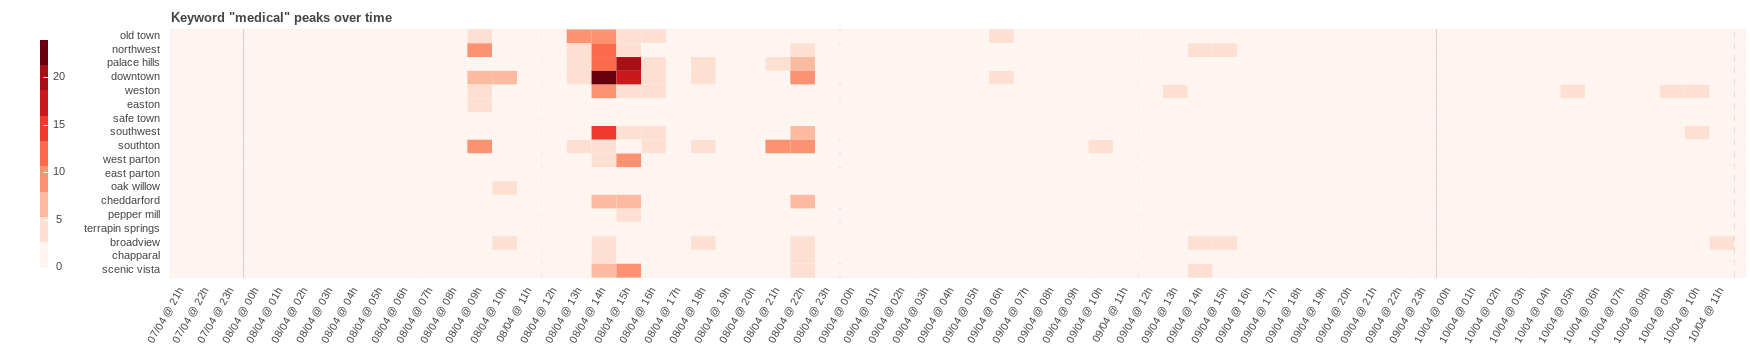
\includegraphics[width=1.00\textwidth]{figs/q2/medical_2_3_heat.png}
        \caption{Medical}
        \label{fig:medical_2_3_heat}
    \end{subfigure}
    \begin{subfigure}[!h]{0.96\textwidth}
        \centering
        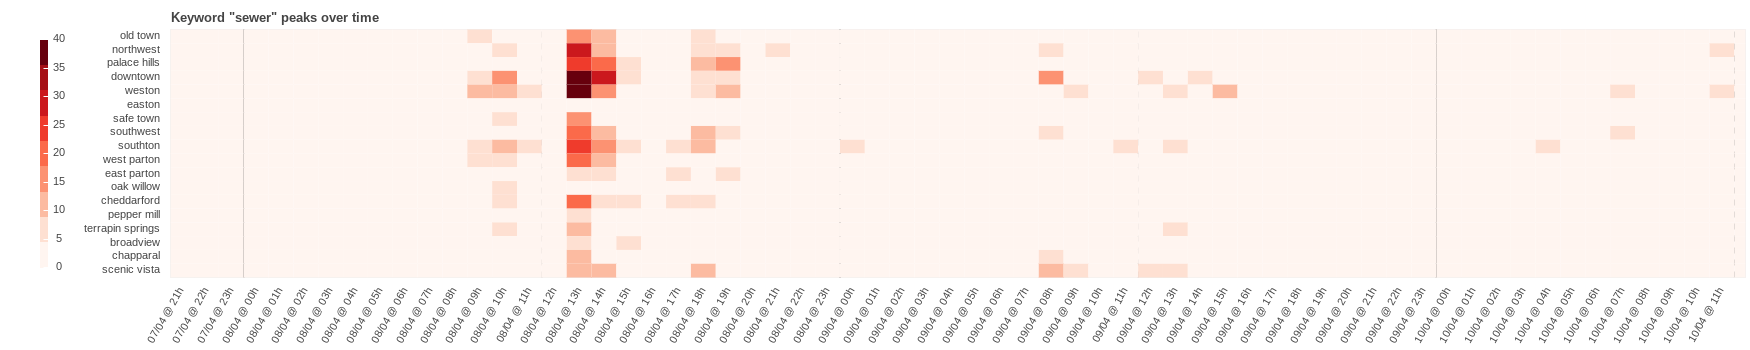
\includegraphics[width=1.00\textwidth]{figs/q2/sewer_2_3_heat.png}
        \caption{Sewer and water}
        \label{fig:sewer_2_3_heat}
    \end{subfigure}
    \begin{subfigure}[!h]{0.96\textwidth}
        \centering
        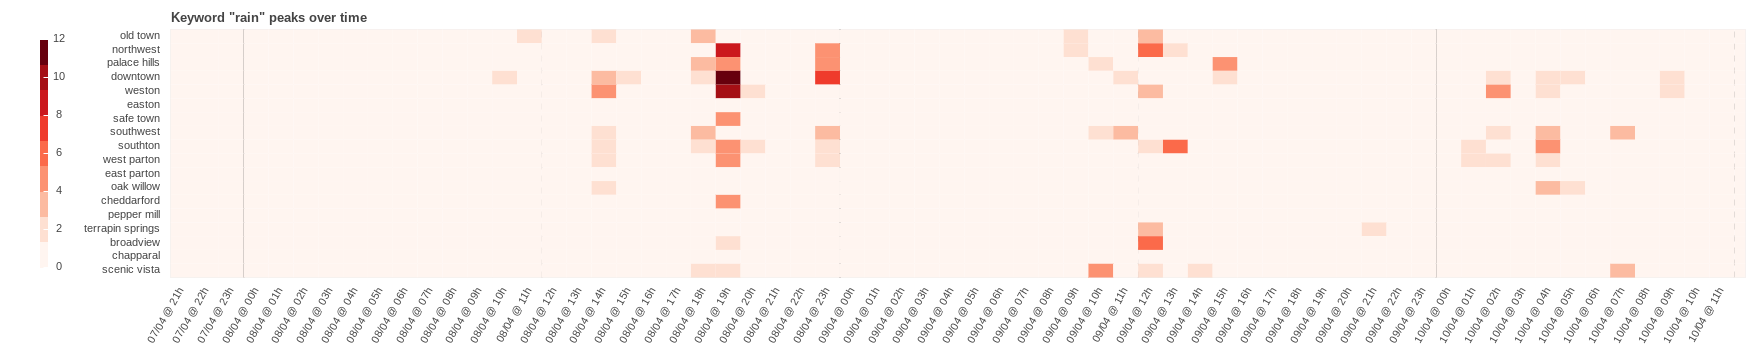
\includegraphics[width=1.00\textwidth]{figs/q2/rain_2_3_heat.png}
        \caption{Rain}
        \label{fig:rain_2_3_heat}
    \end{subfigure}
    \begin{subfigure}[!h]{0.96\textwidth}
        \centering
        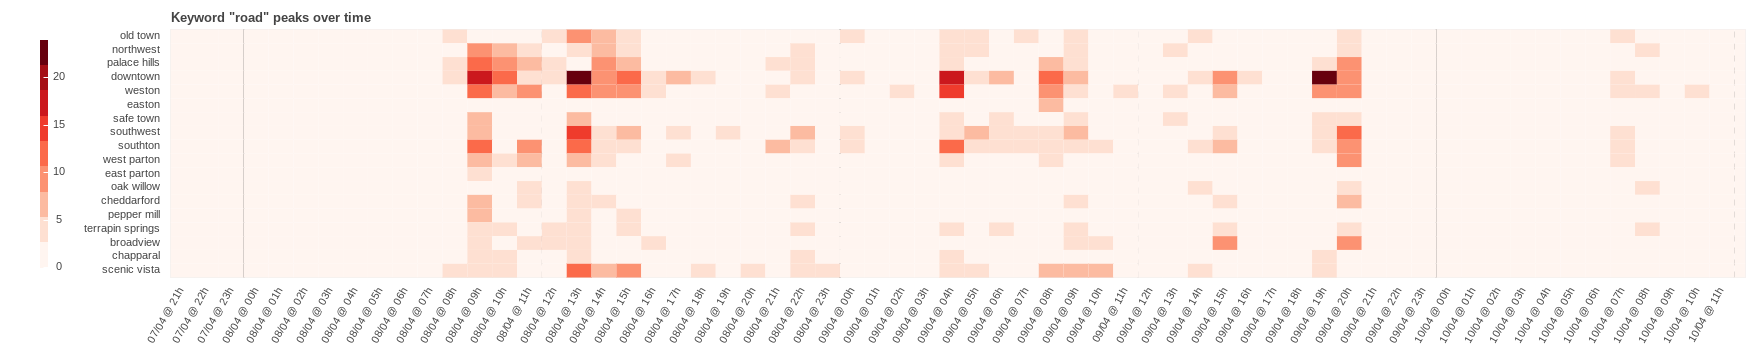
\includegraphics[width=1.00\textwidth]{figs/q2/road_2_3_heat.png}
        \caption{Roads and Bridges}
        \label{fig:roads_2_3_heat}
    \end{subfigure}
    \begin{subfigure}[!h]{0.96\textwidth}
        \centering
        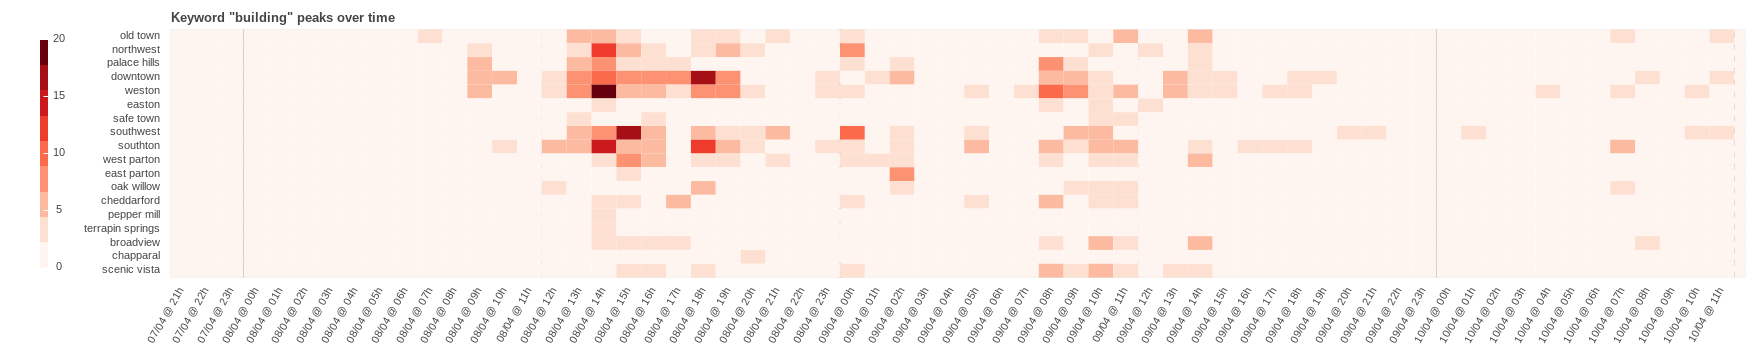
\includegraphics[width=1.00\textwidth]{figs/q2/build_2_3_heat.png}
        \caption{Building}
        \label{fig:building_2_3_heat}
    \end{subfigure}
    \begin{subfigure}[!h]{0.96\textwidth}
        \centering
        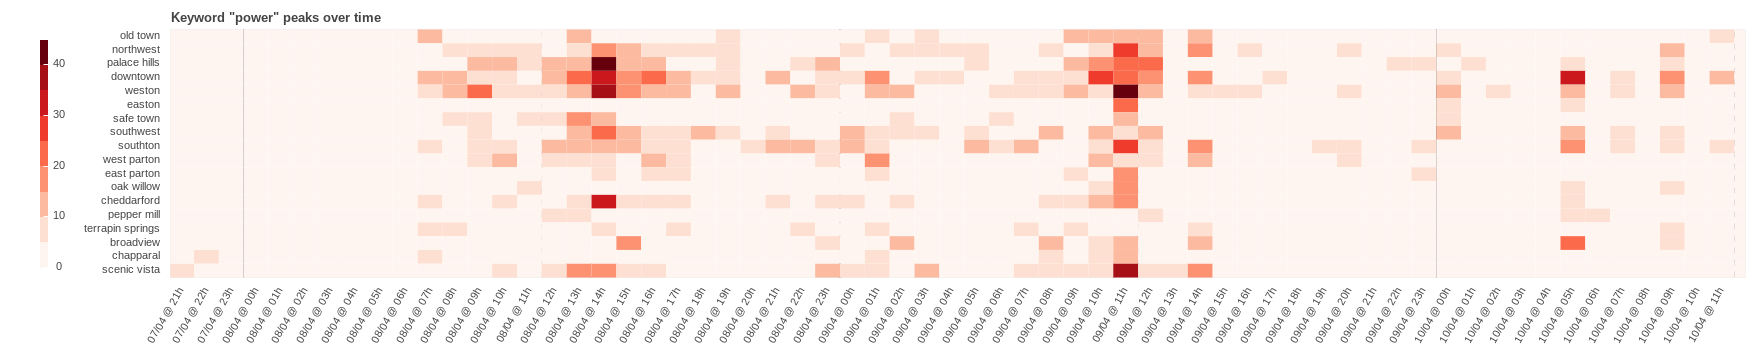
\includegraphics[width=1.00\textwidth]{figs/q2/power_2_3_heat.png}
        \caption{Power}
        \label{fig:power_2_3_heat}
    \end{subfigure}
    \caption{Heatmap of conditions for the two last earthquakes}
    \label{fig:eq_cond_2_3_heat}
\end{figure}

\begin{figure}[!h]
    \centering
    \begin{subfigure}[!h]{0.98\textwidth}
        \centering
        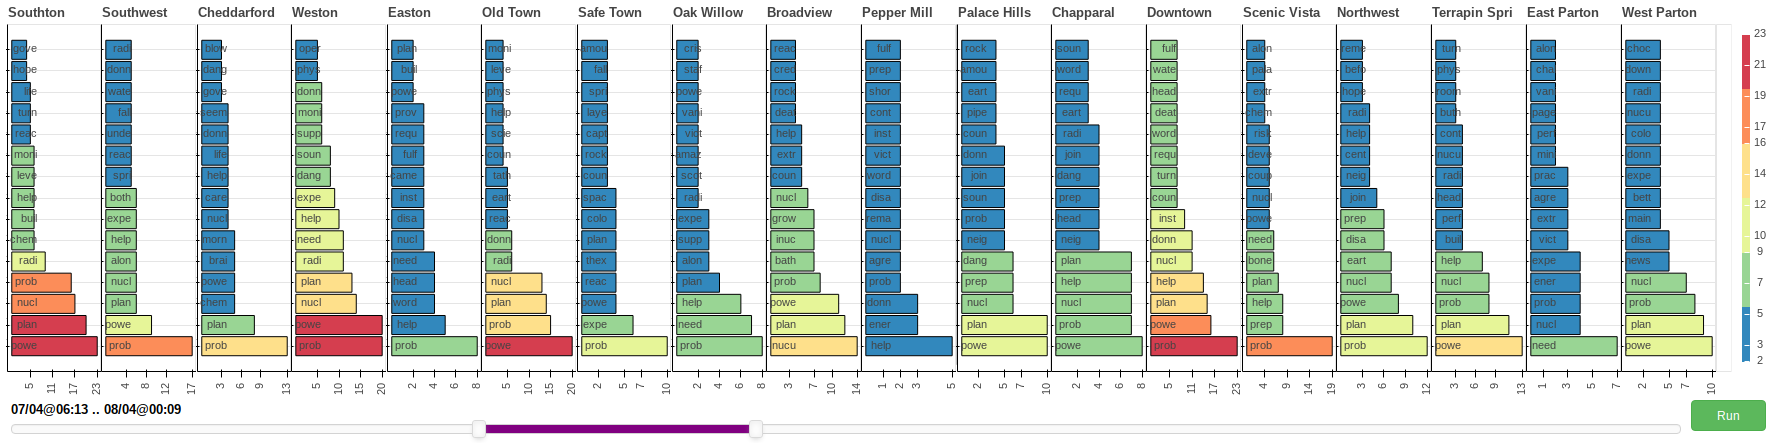
\includegraphics[width=1.00\textwidth]{figs/q2/eq_2_hbar.png}
        \caption{Bar chart for the second earthquake in a 18h time interval from
        Apr 7th at 6:00~PM to Apr 8th at 12:00~AM.}
        \label{fig:eq_2_hbar}
    \end{subfigure}
    \begin{subfigure}[!h]{0.98\textwidth}
        \centering
        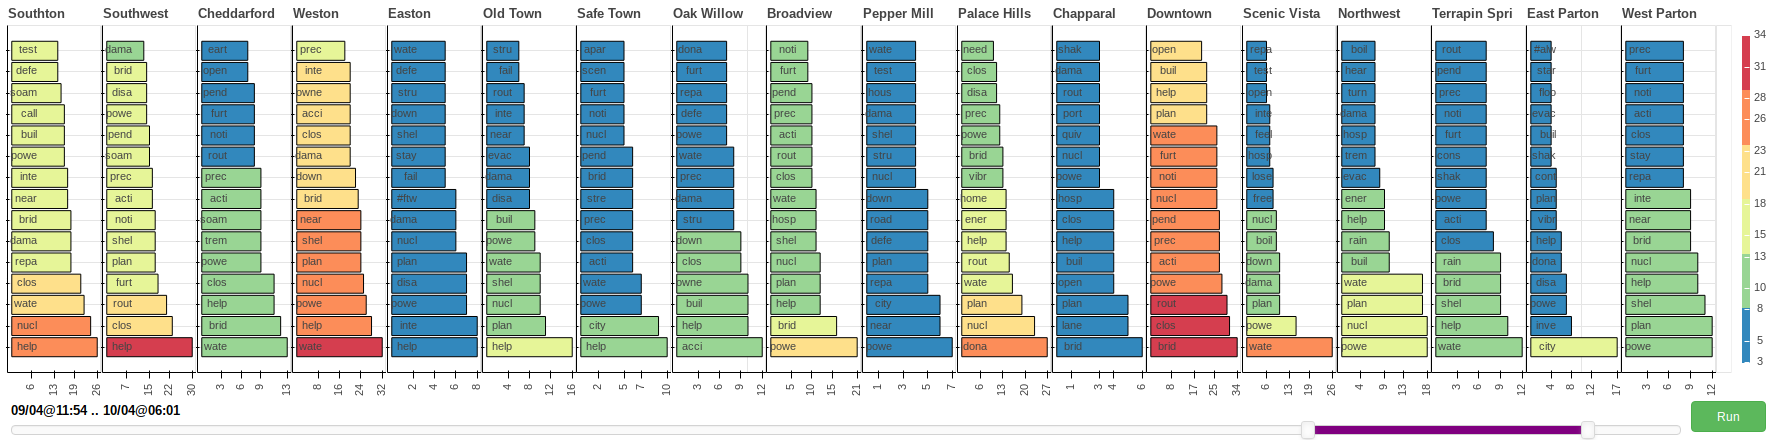
\includegraphics[width=1.00\textwidth]{figs/q2/eq_3_hbar.png}
        \caption{Bar chart for the third earthquake in a 18h time interval from
        Apr 9th at 12:00~PM to Apr 10th at 6:00~AM.}
        \label{fig:eq_3_hbar}
    \end{subfigure}
    \caption{eae}
    \label{fig:eq_2_3_hbar}
\end{figure}

\begin{figure}[!h]
    \centering
    \begin{subfigure}[!h]{0.46\textwidth}
        \centering
        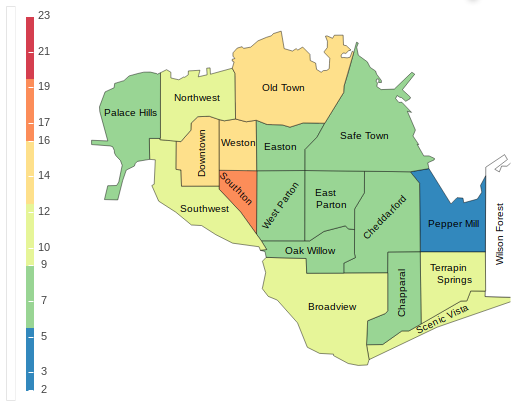
\includegraphics[width=1.00\textwidth]{figs/q2/eq_2_svg.png}
        \caption{Map for the second earthquake. Yellow and orange shades show
        locations where the frequency of tweets is higher. Southton, Downtown,
        Weston and Old Town appear to be, in that order, the neighbourhoods that 
        most need help.}
        \label{fig:eq_2_svg}
    \end{subfigure}
    \hspace{0.75cm}
    \begin{subfigure}[!h]{0.46\textwidth}
        \centering
        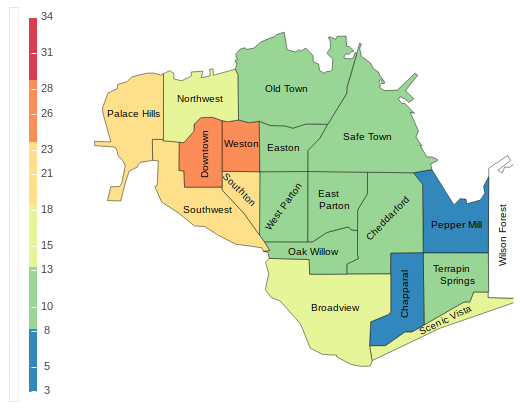
\includegraphics[width=1.00\textwidth]{figs/q2/eq_3_svg.png}
        \caption{Map for the third earthquake. Yellow and orange shades show
        locations where the frequency of tweets is higher. Downtown, Weston,
        Pallace Hills, Southwest, and Southton appear to be, in that order, the 
        neighbourhoods that most need help.}
        \label{fig:eq_3_svg}
    \end{subfigure}
    \caption{St. Himark's SVG maps with blue-to-red colormap for the second and
    third earthquakes.}
    \label{fig:eq_2_3_svg}
\end{figure}

